\chapter{Related Work}
\label{cha:relatedwork}

The P2P (Peer-to-Peer) networking system is an extended concept of network system from the primitive network. The concept of P2P that peers directly connect, and communicate to other peers, is the main distinguishing feature of the distributed network. The ARPANET, historically being the foundation of the internet, can be called as the first P2P system. In 1969, the nodes that are featured in institutes of Stanford University, University of California at Los Angeles, University of California at Santa Barbara, and University of Utah had the first node networking transmission. However, it cannot be signified as being the first P2P network. In 1980, the Usenet is established at the University of North Carolina at Chapel Hill and Duke University \cite{lueg2012usenet}. This has influenced the P2P network structure. Usenet's main distinguishing features are “read and post.” It is composed of the news server and the newsgroups, which are set of newsreaders who are subscribed. The news server pushes the news feed into newsgroups, and when a newsreader submitted the news feed, the news server saves it and exchanges it with other news servers. Its feature is similar to the P2P networking system. Nevertheless, it does not fully implement the features of the P2P networking system. The Usenet does not allow access to the newsreader directly to submit and push. It proceeds only through the news server to exchange the news feed. Around 20 years ago, P2P-based applications have emerged in real world as file sharing or content sharing. Napster is a popular music file sharing application that used the centralized server to point the peer's address, but the transmission data between peers is fully distributed. 

The classic networking architecture is composed of a server and a client. The common networking concept is classified by functionalities as its own roles. In contrast, there is no distinction of each other's roles in the P2P network. That is, the server performs the function of the client, and the client is also the server. P2P networking is the concept of an entity acting as a Servent, used in P2P networks. Servent is an artificial word that is derived from the first syllable of the term server ("\textit{Serv-"}) and the second syllable of the term client (\textit{"-ent"}) \cite{schollmeier2001definition}. Thus, the term Servent expresses its distinct feature. The wide difference between the centralized and distributed network is the utilization of their own resources. The P2P is the Servent-based network; the role of the peer is ambiguous. The participating peers share their hardware resources, such as networking, processing, and storage, and offer their contents.

\section{Overlay network}

The distributed network system implements on overlay networks using Internet Protocol (IP) networks. The P2P as the distributed network is able to widely categorize into structured and unstructured networks.

\subsection{Unstructured networks}

Unstructured P2P networks are randomly set on the overlay network without specific organized structures. It allows to build the peer easily and is able to scale up and down. Peers are able to freely participate and leave the P2P network. Because the unorganized peers are laid on the network, peers are not able to look up the query efficiently. While both peers are laid out, in order to discover the peers, a large number of peers are visited to look up the path. It causes the lost path to occur in routing the peers. The unstructured P2P network does not ensure the lookup result. Freenet, Guntella, FastTrack/KaZaA, BitTorrent, and Overnet/eDonkey2000 are examples of the unstructured P2P network \cite{lua2005survey}.

\subsection{Structured networks}

Contrast to the unstructured P2P network, the structured P2P network is logically organized into a specific method. The peers are set at specified locations according to criteria. When a peer finds content, the target peer who owns the content is deterministically specified. Thus, the search query is efficient in proceeding the discovery of the peer. The network is able to avoid redundant routing traffic to find the target peer, and the lookup function is faster than the unstructured P2P network. The typical example is the Distributed Hash Table (DHT), and it is described in more detail later.

The P2P network system is the basic distributed network concept. From a structural point of view, the P2P network system is able to categorize into the structured and unstructured network on the overlay network. By analyzing both structures' examples in the following sections, we consider both network systems' strengths and weaknesses.

\section{BitTorrent}

After Napster, BitTorrent, which is released in 2001, has been generally the most successful P2P network system. Thus, it spreads the P2P concept among the public. It is a very simple application of file sharing. In 2010, BitTorrent traffic was responsible for about 21.6\% of North American fixed access daily traffic. With Netflix traffic accounting for 22.2\% in the same year, this traffic amount took a significant proportion \cite{sandvine}. Users take advantage of BitTorrent as being the large file sharing in media content. Although the usage is gradually decreasing due to Over-the-top (OTT) media services such as Netflix \cite{netflix}, Hulu \cite{hulu}, Amazon Prime Video \cite{amazon}, and the infringing copyright problems, it is still a popular means of file sharing.

\subsection{Technical framework}

BitTorrent is the typical unstructured P2P network system. These structural features offer advantages of easy scale-up and joining free peers. Also, BitTorrent has the strength to share an enormous amount of any type of data between peers over IP networks. The peers who demand downloading a file join a "swarm" not to access a single server, which has the required file, as a general central server method. Swarm is a set of peers who are interested in the same resource. Swarm has a distinguished member known as "Tracker" who has a list of IP addresses of peers with file resource. Figure 2.1 displays Swarm organization. When the user who wants to upload a file creates a torrent file, the transmittable file is split into numbers of small fragments, and then the created torrent file would be posted on an index site or share with other users. In this procedure, there are different roles of peers in Swarm. The roles of peers divide into Seeds and Leechers. These roles are:

\begin{description}
	\item[Seeds] The peer has whole fragments of the uploaded file.
	\item[Leechers] The peer has at least one fragment. However, it has not completed correcting fragments yet.
\end{description}
	Seeds : The peer has whole fragments of the uploaded file.
	Leechers : The peer has at least one fragment. However, it has not completed correcting fragments yet.
Swarm consists of Tracker, Seed, and Leecher. Tracker has a list of Seeders and Leechers with information and offers only the Seeds and Leechers' address to the participating peers in the Swarm. They share the own fragments with other Leechers. As a Leecher has completely gathered all fragments, it becomes a Seed. If there is not even one Seed in the Swarm, Leecher never completes a download file. Any Peer is able to join the Swarm. However, they must obtain a torrent meta-data file extended .torrent. The torrent meta-data file contains the Tracker's URL and information of the target file, such as the name of the file, the file length, the length of the fragment of the file, and the SHA-1 hash code for each fragment. BitTorrent using the torrent meta-data file verify data integrity, deficient fragments, and connection to the Tracker. 

\begin{figure}[!ht]
	\centering
	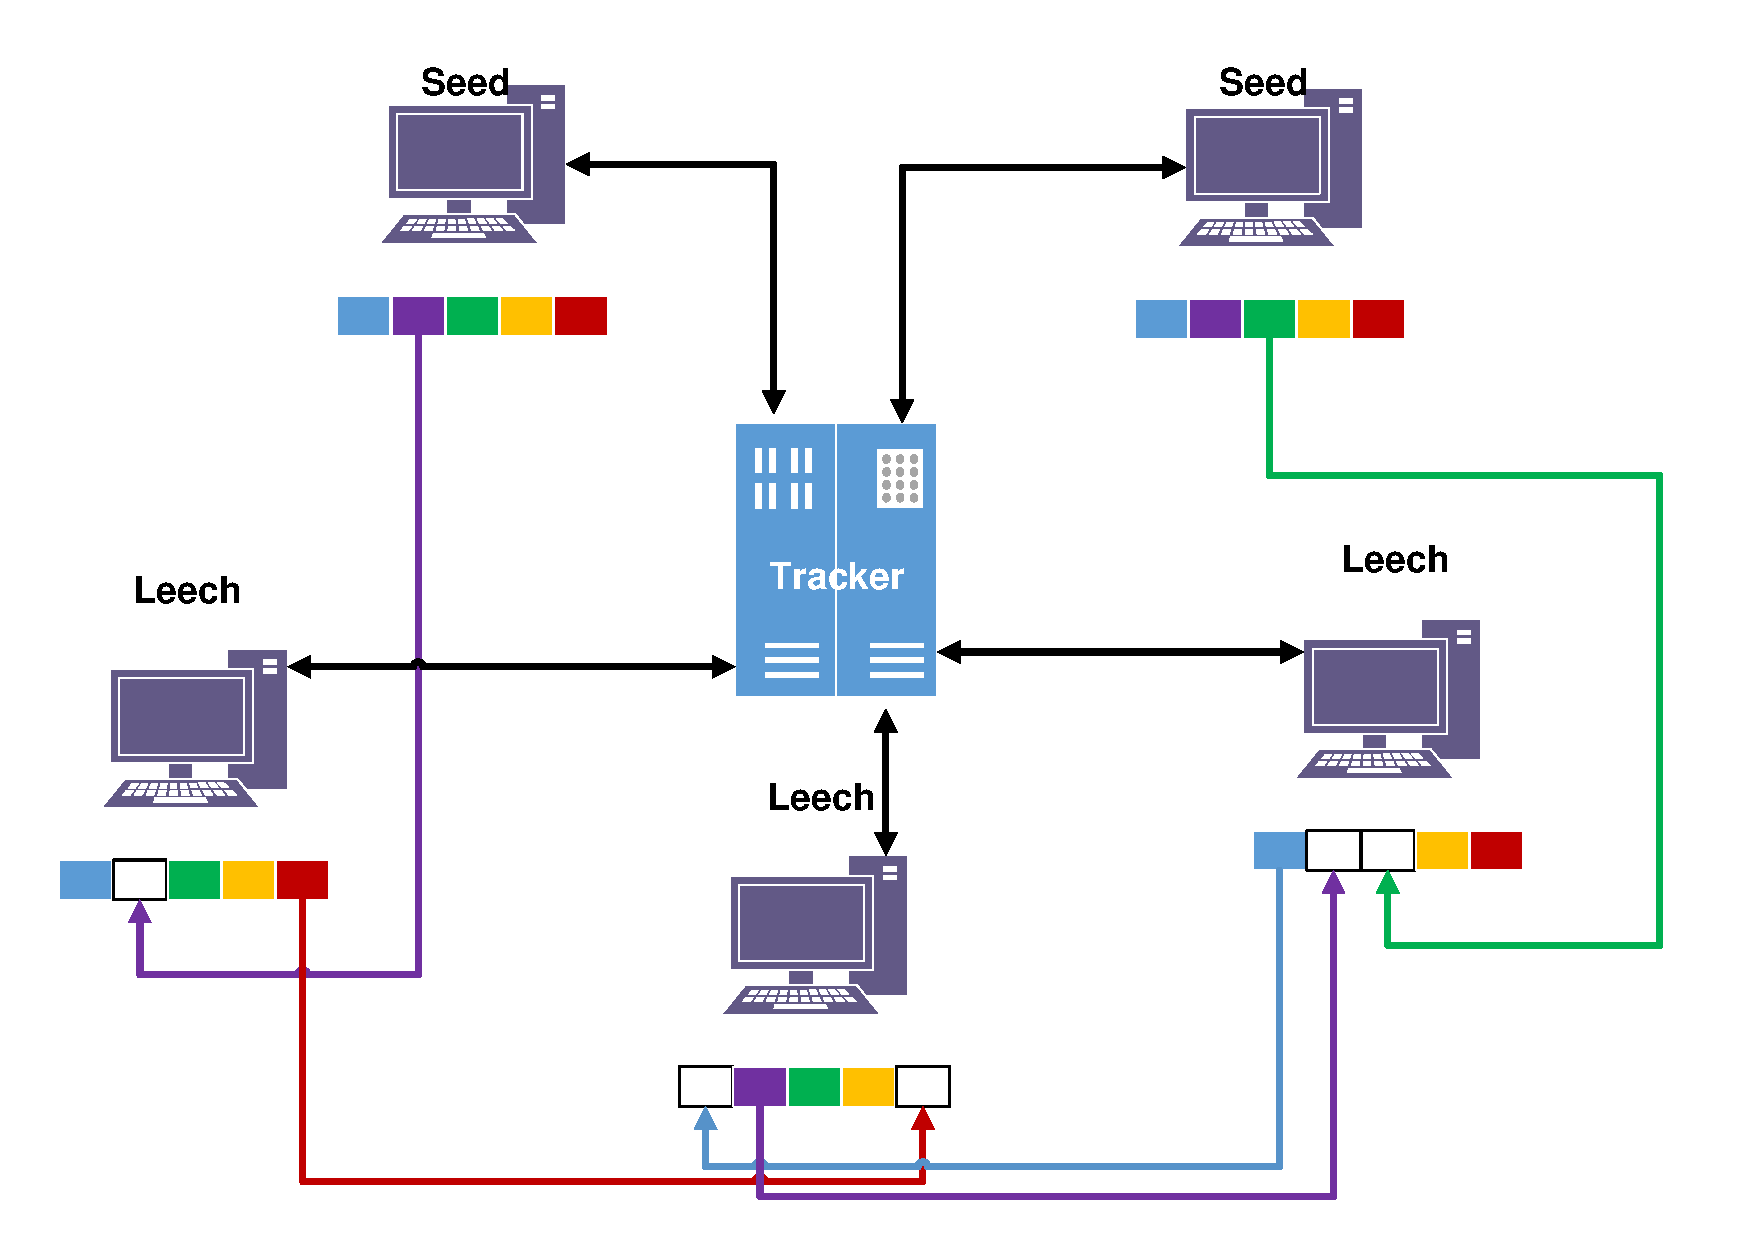
\includegraphics[width=0.5\textwidth]{images/fig_2_1.pdf}\\
	\caption{Overview of Swarm}
	\label{fig:Swarm}
\end{figure}

The main data transfer in the BitTorrent process occurred at the connection between peer and Tracker, and peer and peer. The two connections use different protocols. Peer-Tracker connects through HTTP. A downloader requests to Tracker what file it wants to download through the torrent meta-data over an HTTP network \cite{chokkalingam2004bittorrent}. Peers transfer data over the TCP network \cite{chokkalingam2004bittorrent}. They make a pipeline, and they then establish a connection via a handshake. BitTorrent has adopted distributed file sharing, where peers transfer divided fragments each other,  avoiding the problem of existing server-client-based platforms such as traffic congestion. It is anticipated in being continued to use a popular extensive file sharing application.

\section{Distributed hash table}

The structured P2P network deploys logically participating peers on the overlay network. The peers are located according to specific criteria. In this location procedure, a Distributed Hash Table (DHT) helps to determine the location and store peers. There is a difference between structured and unstructured systems. The main feature of DHT is a Key-Value paired, which is similar to the hash table. Because of this feature, its algorithm is a derivative of the hash table. Figure 2.2 demonstrates an overview of DHT. 

\begin{figure}[!ht]
	\centering
	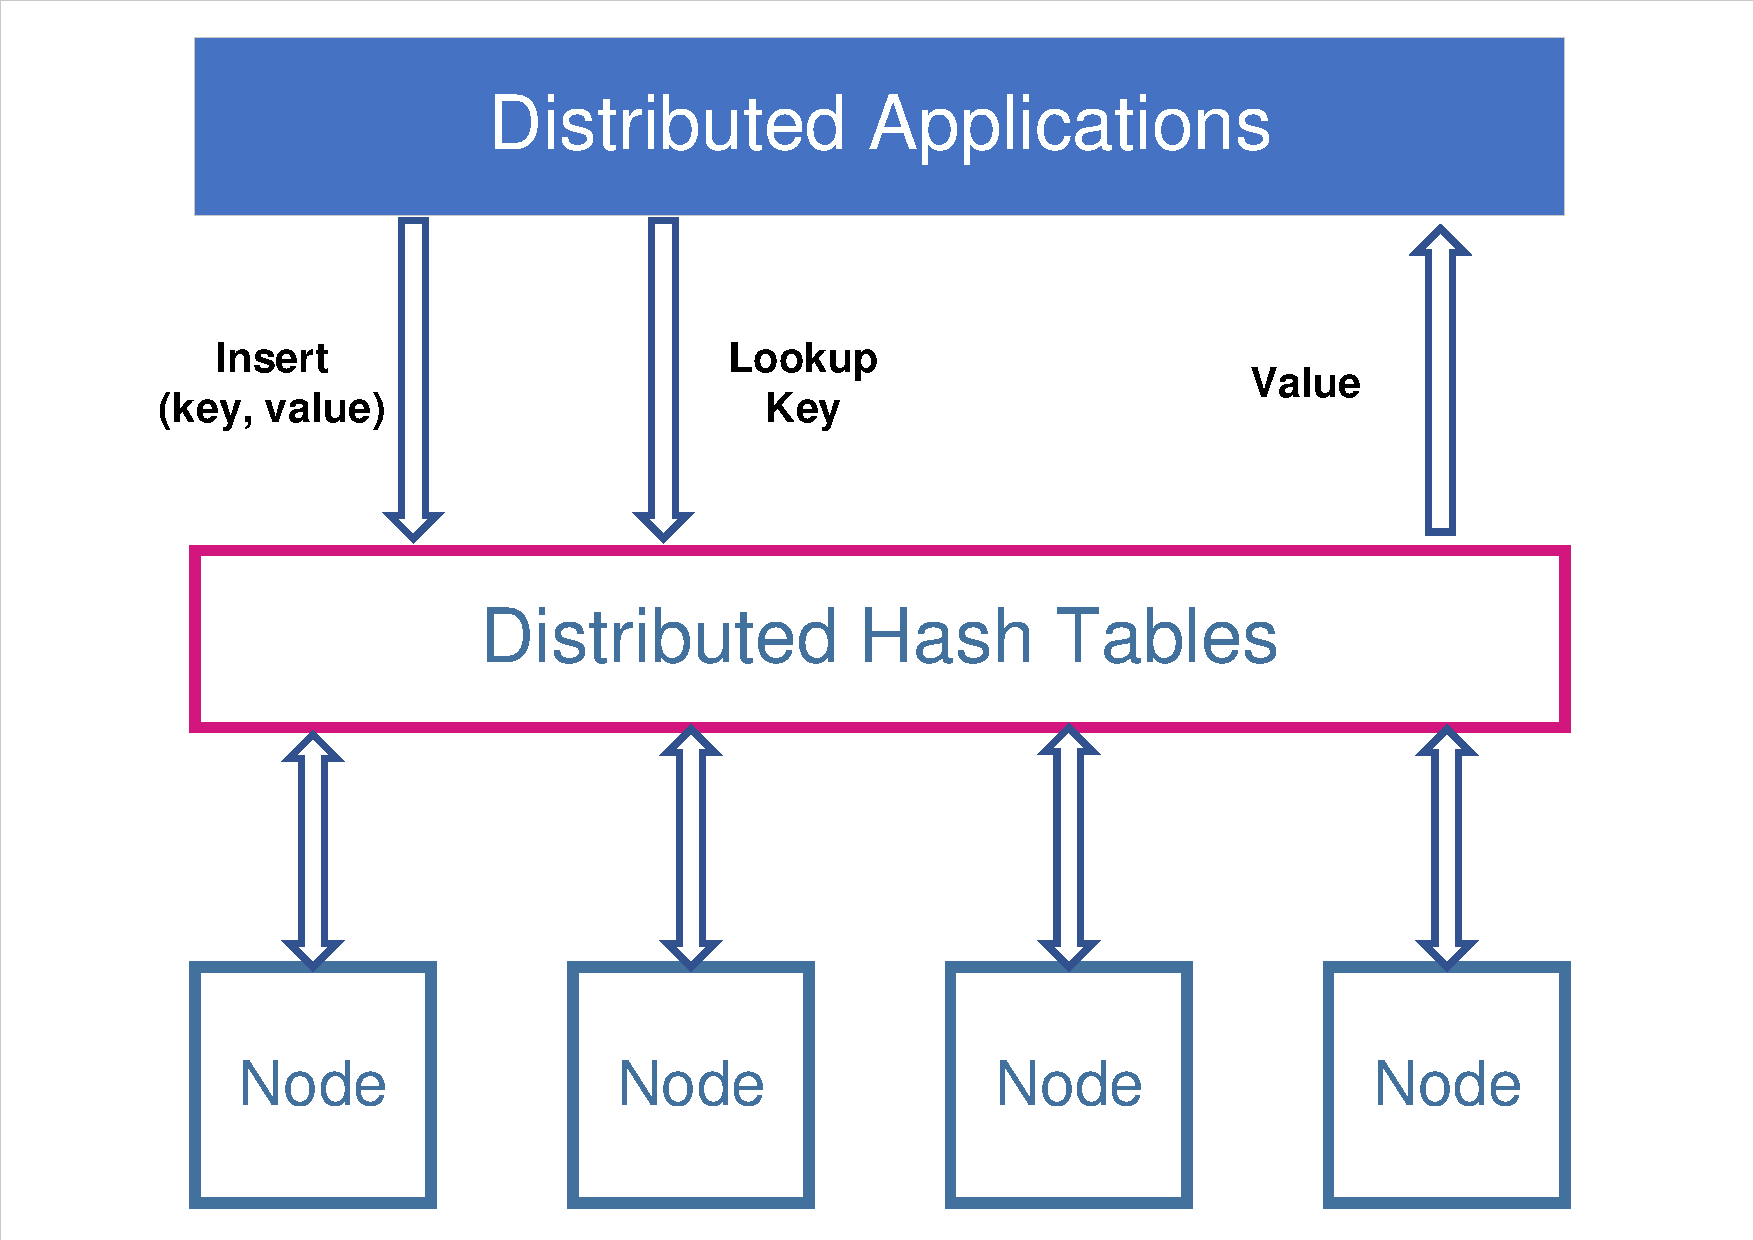
\includegraphics[width=0.5\textwidth]{images/fig_2_2.pdf}\\
	\caption{Overview of DHT}
	\label{fig:DHT}
\end{figure}

The factors, which are key and value, are used in a lookup service. If the identifier uses the insertion of DHT or unique key during search process, associated values related to DHT can be found.  DHT can handle the resource that any data types, such as peers, documents, binary data, addresses, are available. The given key is generated using a hash function such  as SHA-1. The generated hashed key is the set of m-bit strings. The hashed key k is mapping the values like <k, data>. The data of paired Key-Value propagate to participating peers through the overlay network. When a peer retrieves a resource, the resource's key generates hashed key k and then a lookup message with k routes to associated peers. If the value mapped with k existed, it will be returned. The core operations of DHT are this insertion and lookup. 

In P2P network systems, DHT has advantages such as having large numbers of peers who can join the network. The peers are joined in a set of small numbers of other peers, called the neighbor or routing table. The neighbor is determined through an underlying algorithm. It is called the network’s topology. In the DHT topology, the concept of distance is an important property. Each peer has an own identifier as a key, and according to the distance between peers, the neighbor is determined. When a message is routing in the P2P network, it will forward to a certain neighbor and then arrive at the destination peer. According to routing algorithms, there are various DHTs such as Kademlia \cite{druschel2003peer}, CAN \cite{ratnasamy2002routing}, Pastry \cite{rowstron2001pastry}, Chord \cite{stoica2001chord}, and Tapestry \cite{zhao2001tapestry}.


\section{Kademlia}

P2P network system allows joining a large number of peers. Thus, the system should control them efficiently. The structured overlay network system organizes the network topology using DHT. Kademlia is one of the implementations of DHT using exclusive or (XOR or $\oplus$). It is designed in 2002 by Petar Maymounkov and David Mazières. It follows a basic DHT operation. Key and Values are primary entities. Therefore this 2-tuple are paired such as <$key, value$> tuple. The key that has m-bit key space is given randomly, and then such key encrypted by hash function; the basic Kademlia uses SHA-1. A peer is using the key for a unique identifier. As well as other DHTs, the Kademlia algorithm locates the values through the given key. The distance among peers is a specific character of DHT. In Kademlia, such distance is calculated through the XOR metric. When we consider the m-bit key being 4-bit long, the examples can be computed by the bitwise XOR, producing the following result.

\begin{description}
	\item \textit{\textbf{Distance}}(0000, 1111) = 1111 = 15
	\item \textit{\textbf{Distance}}(1010, 1111) = 0101 = 5
	\item \textit{\textbf{Distance}}(0011, 1110) = 1101 = 13
	\item \textit{\textbf{Distance}}(0011, 1010) = 1001 = 9
	\item \textit{\textbf{Distance}}(0011, 0010) = 0001 = 1
\end{description}

The closest peers are the peer ID 0011 and the peer 0010, and the distance is interpreted as an integer. Formally \cite{lavoie2017xor}:

$$x_{i} = \left\{0, 1\right\}
$$
$$X=\left(x_1,x_2,x_3,\ldots,\ x_b\right)
$$
$$x_i\oplus y_i=0\ if\ x_i=y_i,\ 1\ otherwise
$$
$$d\left(X,Y\right)=\ \sum\nolimits_{i}^{b}{2^{i-1}(x_i\oplus}y_i)
$$

The entire space of the identifier consists of which the value is binary keys from 000...0 to 111…1. The values of keys are able to be expressed as a binary tree. The binary tree is illustrated in Figure 2.3. Each peer comprises a list for each bit of ID; m-bit ID stores m lists, called a bucket. Kademlia DHT forwards a message such as a lookup to other peers in the bucket. The pointed ID of the target peer of i-th bucket is matched with the peer ID of m-i bits. For example, when the peer ID is 0011, the first bucket points 0010. The three bits of the prefix of the target peer have matched the peer ID. In Figure 2.3, the second bucket should point to the peer 000x. However, there is no target ID. It means, in that space, no peer has been connected yet. The third bucket should point to the ID 01xx. There are peer 0101 and peer 0110. Peer 0110 has a logically shorter distance than peer 0101. As a result, the third bucket stores the peer 0110. At last, the fourth bucket points to the peer 1010 as the same operation. This significant concept of the bucket supports Kademlia’s functions such as lookup and location service.

\begin{figure}[!ht]
	\centering
	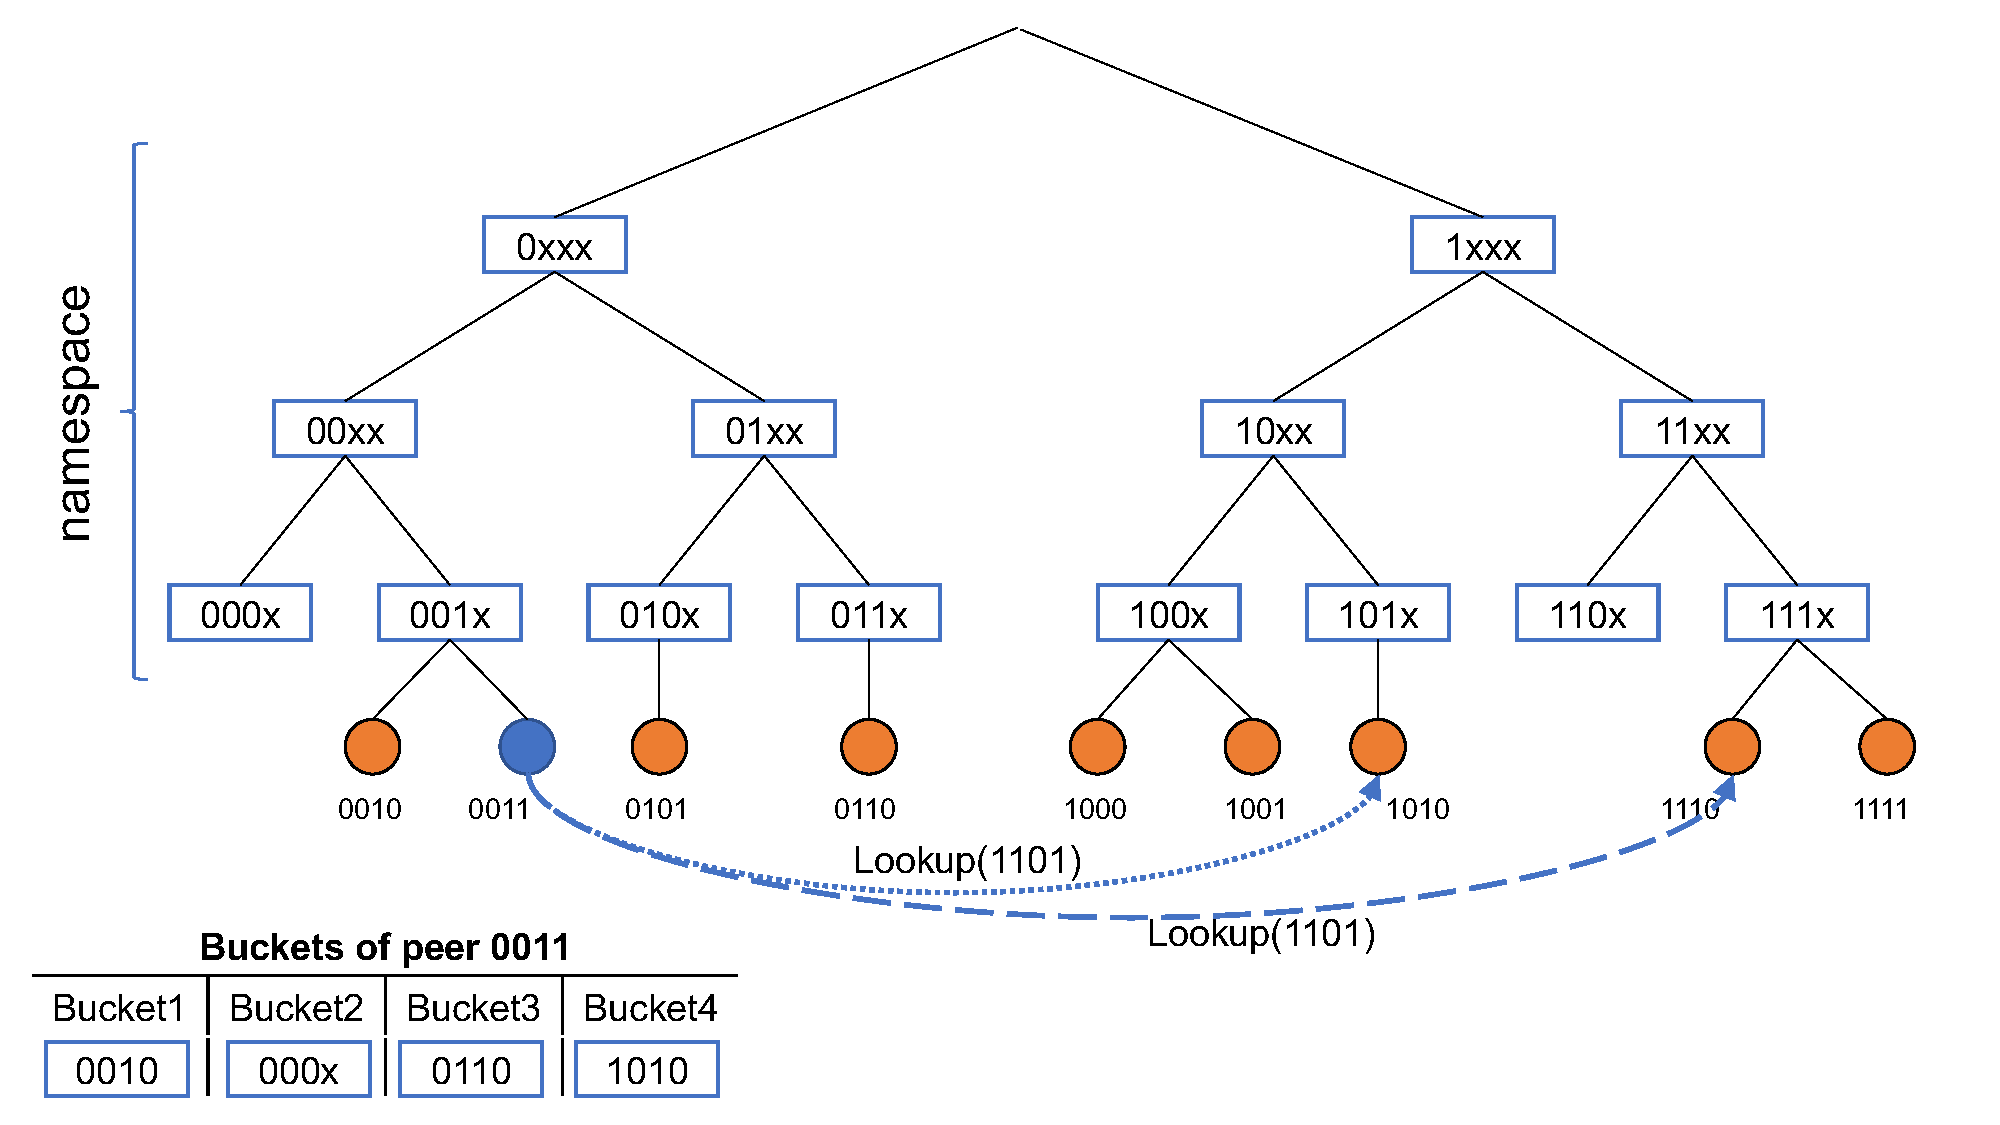
\includegraphics[width=0.5\textwidth]{images/fig_2_3.pdf}\\
	\caption{Kademlias’s binary tree}
	\label{fig:kademlia}
\end{figure}

\subsection{Lookup service}

The Kademlia algorithm uses the distance among peers, which is computed by an XOR metric. The lookup service figures out the shorter distance using the triangle inequality. When we consider to lookup the peer 1110, the recipient peer 0011 calculates peers its in an own bucket. The fourth bucket that points to peer 1010 is in close proximity to the requesting peer. The recipient peers the query to peer 1010, and then peer 1010 retrieves the requesting peer in its bucket as same as the first procedure between the recipient peer and the peer in the fourth bucket. As the requested peer is found, the recipient peer 0011 receives a result of lookup from peer 1101. In Figure 2.3, the procedure is illustrated with the dotted line. The Kademlia’s routing performance, in comparison with other structured overlay DHT network algorithms, can increase using the bucket by m-bit prefix function because the hops per lookup are reduced from ${log}_2{n}$ to ${log}_{2^m}{n}$ \cite{druschel2003peer}.

\subsection{4.2.	Kademlia protocol}

The Kademlia peers communicate through specific messages. The Kademlia DHT has four RPC messages: PING, STORE, FIND\_NODE, and FIND\_VALUE.

\begin{description}
	\item[PING ] The peer sends this RPC to other peers to verify the condition of the peer, whether it is online or not.
	\item[STORE] This RPC includes <$key, value$> pair for a store in a peer.
	\item[FIND\_NODE] The recipient peer takes a return message from the buckets. The message contains information about peers. It is the closest to the requested peer ID.
	\item[FIND\_VALUE] It is similar to FIND\_NODE operation. The recipient peer will take a return value that the key of paired value is matched with the requested key if the corresponding ID is stored.
\end{description}

All of RPCs involve a lookup service. A participating peer must have a procedure to locate the closest nodes. It is imperative in Kademlia. In Section 4.1, we describe the lookup service.

Kademlia DHT is a flexible, reliable, and robust structured P2P network system. The key-value paired concept supports the system builds the simple DHT architecture. Such XOR-based metric topology gives the advantage of increasing the routing performance. Kademlia is one of the suitable DHT algorithms for filesharing.

\section{QUIC protocol}

The transport layer offers a communication service among hosts in a computer network. The host transfers data through transport protocols. Transmission Control Protocol (TCP) is connection-oriented, and User Datagram Protocol (UDP) that is connection-less based is a well-known transport protocol. Both protocols are suitable for web applications, and they are today widely used. However, with the development of internet service, applications require enhanced performance. In 2015, at the Internet Engineering Task Force (IETF), a newer HTTP/2 standard is released. It is a major revision of HTTP/1.1. It supports decreasing latency to raise speed of loading pages, multiplexing streams over a single TCP connection, pipelining, and header compression. However, it is still using connection-oriented TCP. It is not able to avoid the problem of Head-of-Line (HOL) blocking, that is, the packet loss problem at the end-user; It occurs when data are transmitted to the end-user from multi-paths, there happens traffic congestion, and then any packets can be dropped. Moreover, TCP has limitations for rapidly handling massive internet traffic in web pages and web applications. Therefore, a necessity for a novel transport protocol emerged. 

As a result, Google developed a novel transport protocol QUIC in 2013 (Quick UDP Internet Connection) and implemented it in their web browser called Chrome. Since 2018, the IETF is working on the HTTP mapping over QUIC for HTTP/3 standard. QUIC’s goals are briefly as follows \cite{experimentingwithquic}.

\begin{description}
	\item High security similar to TLS (Transport Layer Security).
	\item Fast (often 0-RTT) connectivity similar to TLS Snapstart combined with TCP Fast Open.
	\item Packet pacing to reduce packet loss
	\item Packet error correction to reduce retransmission latency
	\item UDP transport to avoid TCP head-of-line blocking
	\item A connection identifier to reduce reconnections for mobile clients
	\item A pluggable congestion control mechanism
	
\end{description}

\subsection{Connection establishment}

QUIC relies on UDP instead of TCP. TCP needs the specific connection establishment procedure from a client to a server, called a handshake. The handshake procedure in TCP requires three Round Trip Time (RTT) phase:

\begin{description}
	\item A client who wants to establish a connection, sending a SYN message to a target server.
	\item The server that responses to the client with a SYN ACK message.
	\item The client who responses to the server with a ACK message.
\end{description}

Then, the connection establishment is completed. Moreover, encrypting data using the TLS protocol require one more RTT. However, QUIC does not require the handshake procedure as the same as the TCP handshake. It uses to initiate a version negotiation. A client who sends the packets should include the version flag, and then a server sets the protocol version through the flag of received packets. The set version keeps during the connection. When the server responses to the client, it must send the crypto handshake data. As a result, crypto and transport handshakes operate at the same time. Therefore, QUIC’s RTT in the connection establishment is able to reduce to 0-RTT. In Figure 2.4, the comparison handshakes of QUIC, TCP, and TCP+TLS are shown.

\begin{figure}[!ht]
	\centering
	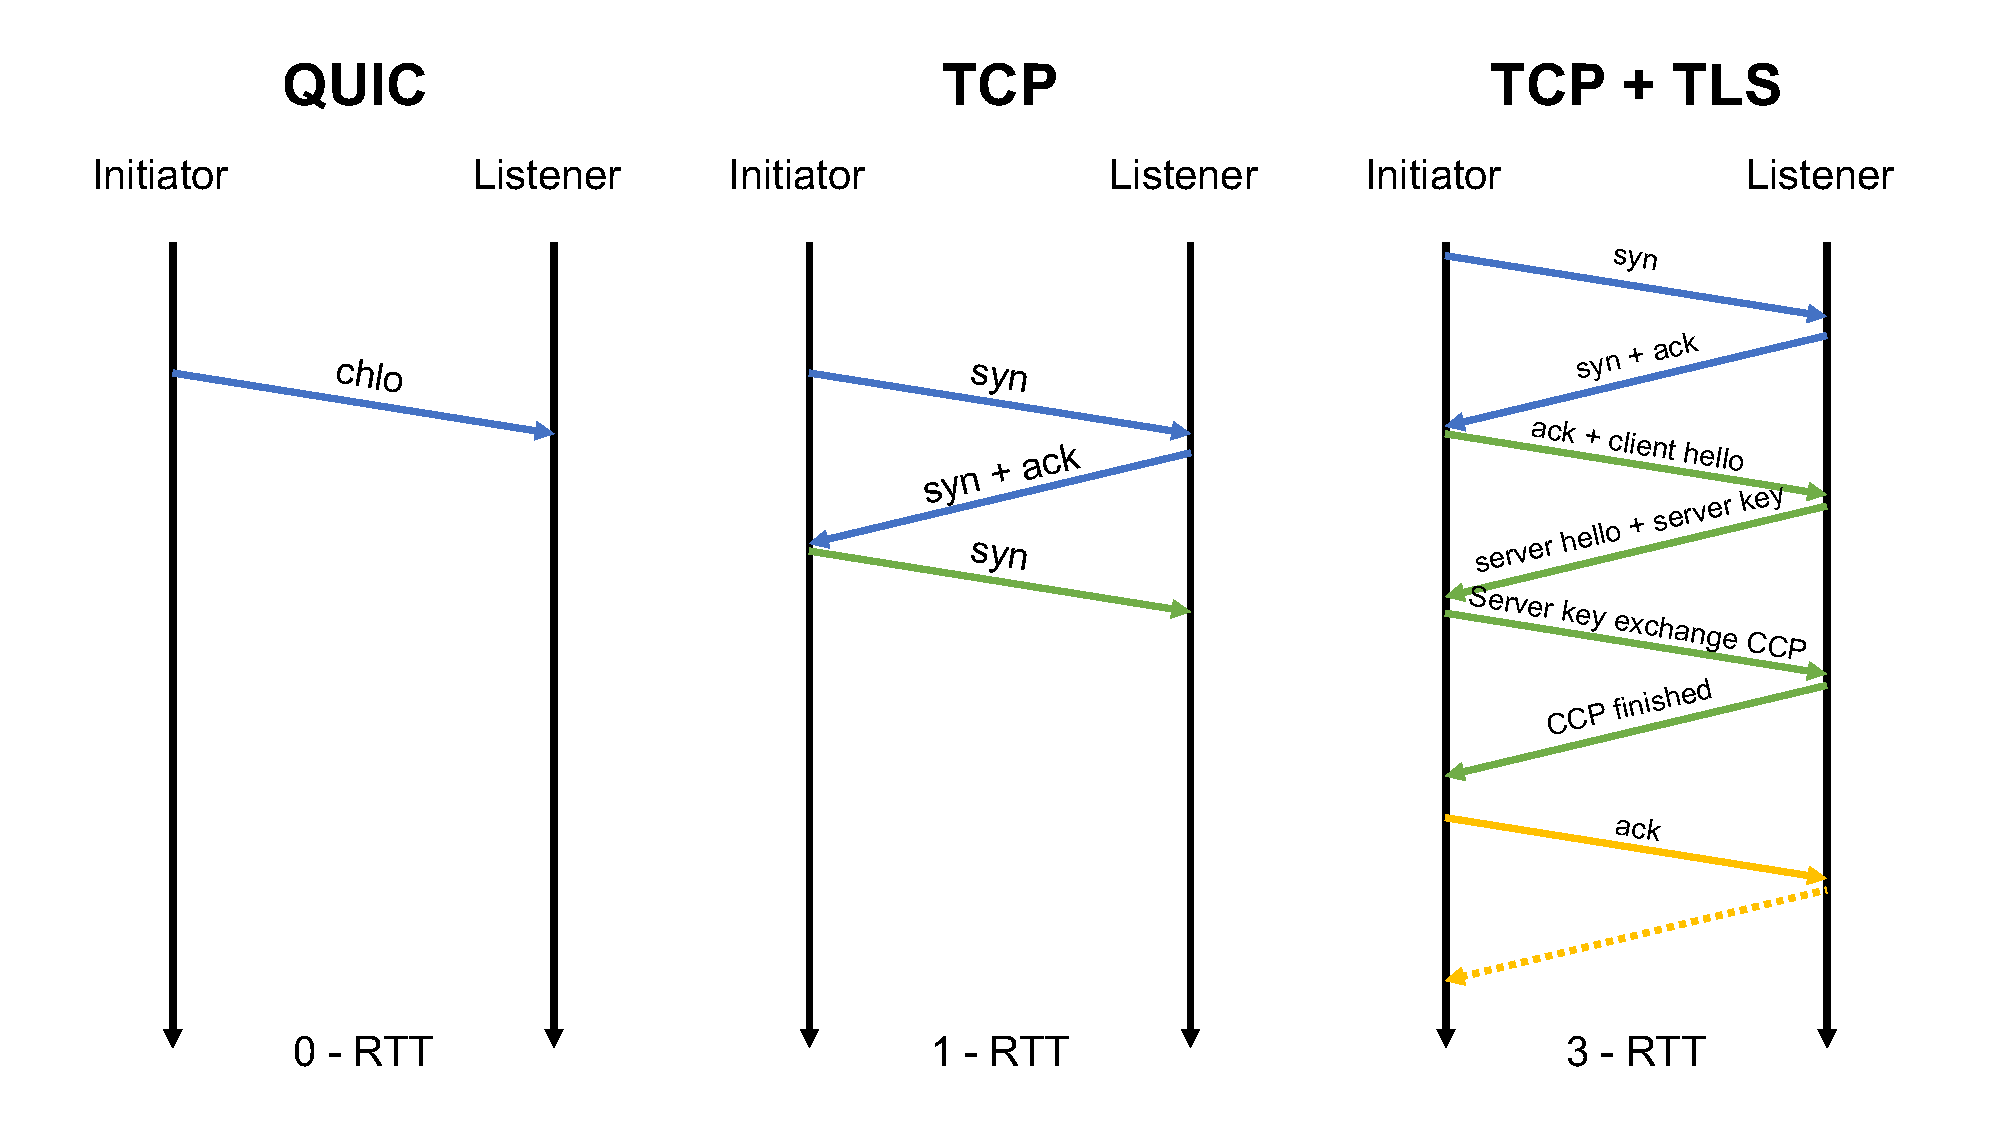
\includegraphics[width=0.5\textwidth]{images/fig_2_4.pdf}\\
	\caption{Comparison handshakes of QUIC, TCP, and TCP+TLS}
	\label{fig:RTT}
\end{figure}

\subsection{Congestion control}

QUIC provides a richer pluggable congestion control than TCP. QUIC gives different sequence numbers to packets; the original packet and retransmitted packet have different sequence numbers, and consequently, it is able to avoid retransmission ambiguity. QUIC supports larger NACK in ACK up to 256 bit than TCP 32 bit SACK. Thus, QUIC has more space for reordering packets. It takes advantage of enhanced congestion control \cite{drafttsvwgquicprotocol02}\cite{nalawade2018comparison}.

\subsection{Error control}

QUIC adopts an XOR-based Forward Error Control (FEC) scheme, in which an FEC packet includes a parity packet to check the error. When a receiver detects packet loss, the lost packet is recovered from the FEC packet without retransmitting the lost packet.

\subsection{Connection migration}

QUIC is recently designed for the future HTTP protocol. Many users can access websites and web applications via a mobile device while they move somewhere. Thus, the client’s IP address is able to be frequently allocated newly during changing wireless networks or handover of the mobile network. In TCP, a connection should reestablish after the set time. However, QUIC utilizes a unique connection identifier. Therefore, even if a user connects to another network and causes the reallocation of IP address, the reconnection can be established again using the identifier.

QUIC has adopted the many features of TCP. Therefore it has similarities between QUIC and TCP. It is able to complement the weakness of TCP and improve performances. However, it is still working for mapping newer HTTP/3. Currently, it can be used for restricted areas such as adopted web browsers and some supported servers. When it is completed, it can become one of the major protocols.
